\chapter{ Resultados Experimentais }
\label{cap:resultados}
\section{Experimentos}



\subsection{Modelos de Aprendizado de Máquina}


Em um primeiro momento, o problema é tratado como de Aprendizado Automático para
dados não temporais. Para esses modelos como Redes Neurais, Árvores de Decisão e Regressões
Lineares, separamos os dados em treino e validação, normalizamos as variáveis e
treinamos os modelos. 

\subsubsection{Divisão dos dados entre treino e validação}


A divisão entre dados de treino e validação é feita da maneira padrão com
modelos de Aprendizado de Máquina, separando-se $80\%$ dos dados para treino e
$20\%$ para validação, i.e. testar o poder de generalização dos modelos. 

\begin{figure}[H]
  \centering
  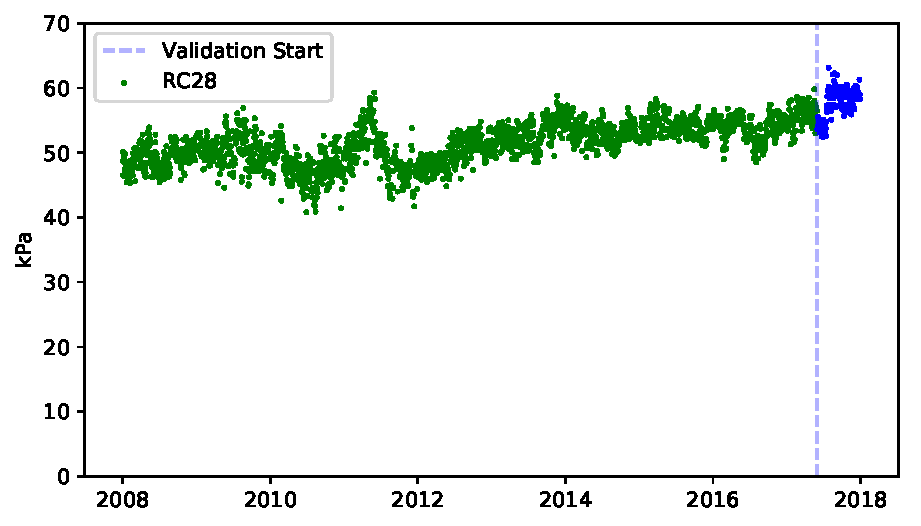
\includegraphics[width=0.9\columnwidth]{train_dev.pdf}
  \caption{Divisão do dataset para a saída RC28, os pontos verdes foram usados para
    treino e os pontos azuis usados para validação.}
  \label{fig:divrc28}
\end{figure}

Foram usadas implementações dos modelos fornecidos pela biblioteca Sklearn.
As avaliações de RMSE de todo o conjunto de validação estão apresentados por modelos na Imagem~\ref{fig:mlmodels}.  

\begin{figure}[H]
  \centering
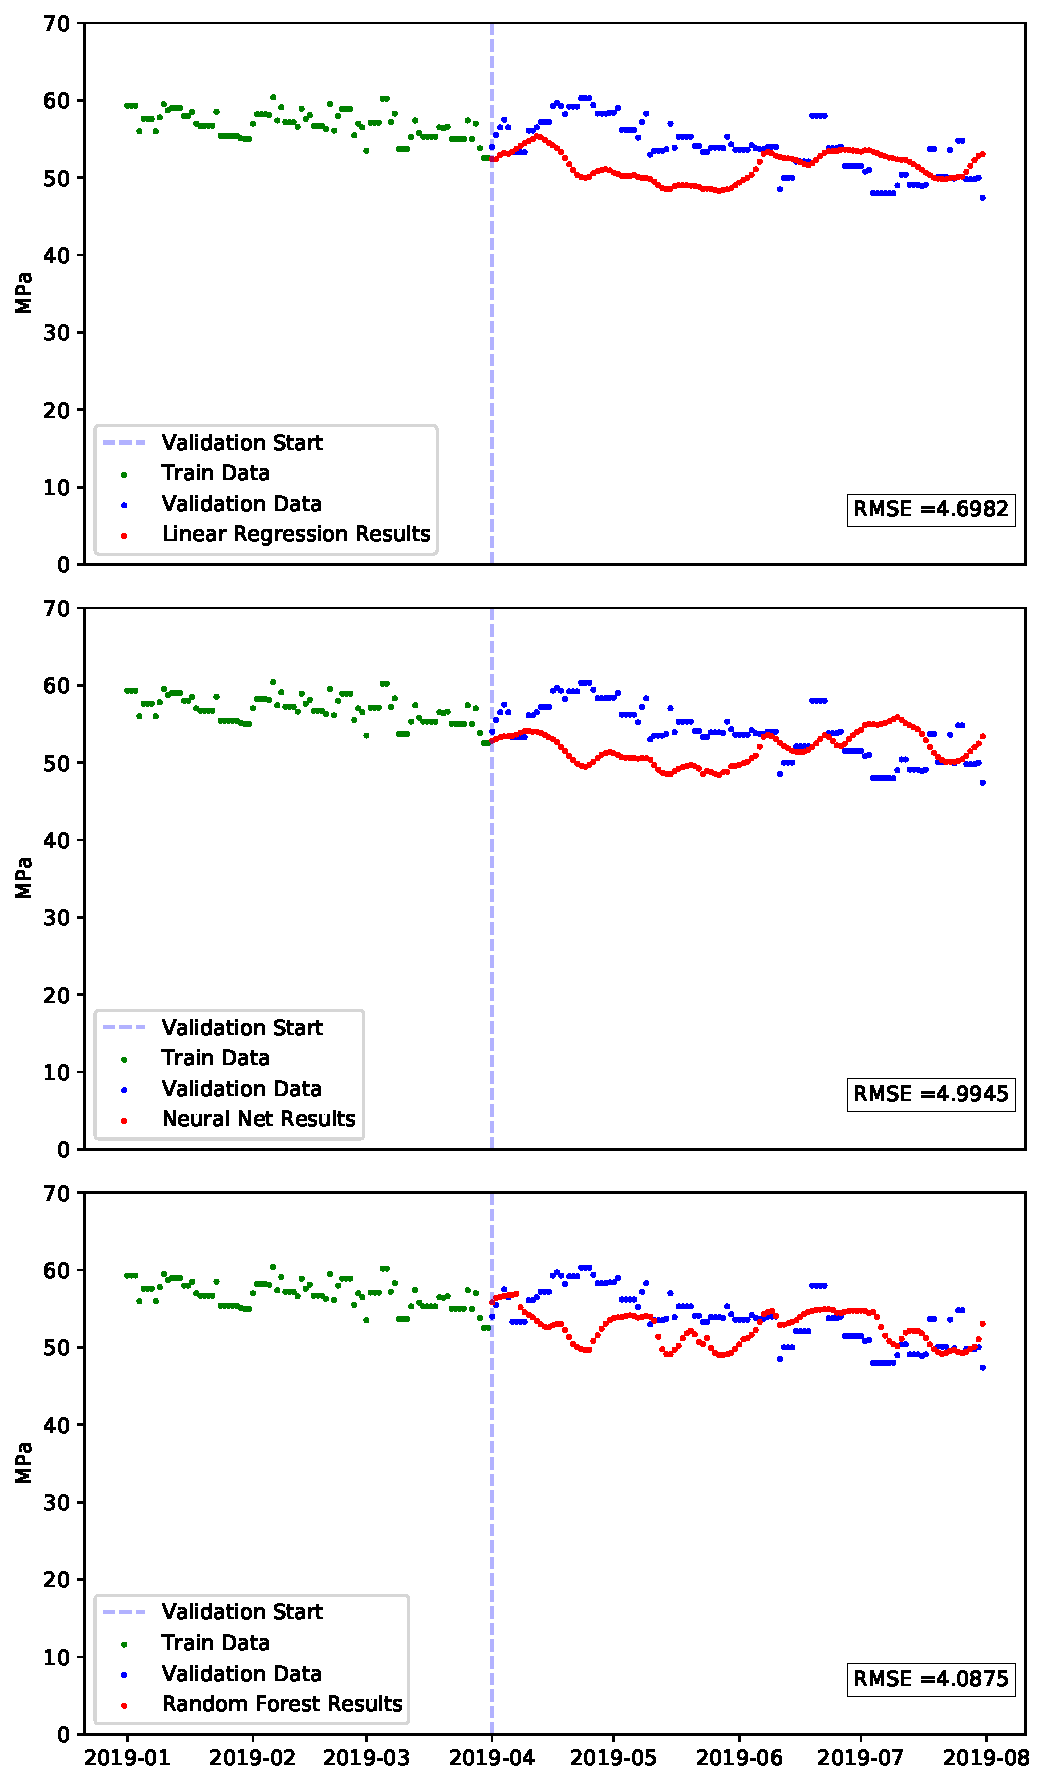
\includegraphics[width=0.9\columnwidth]{mlmodels.pdf}
\caption{Predições nos dados de validação nos experimentos com modelos não-temporais. }
\label{fig:mlmodels}
\end{figure}

Na Tabela~\ref{tb:rmse_lin} reportamos os erros para predições imediatamente
após o fim do último dia de dados usados para treino. Iremos mostrar o
erro para o dia seguinte, três dias depois e então uma semana após o último dia
de dados usados para treinamento.

\begin{center}
\begin{table}[htbp]
\caption{RMSE por horizonte de predição.}
\centering
\begin{tabular}{rr}
\hline
 Regressão Linear & RMSE\\
\hline
24h & 2.94\\
3d & 0.13\\
7d & 5.43\\
\hline
Rede Neural & RMSE\\
\hline
24h & 3.70\\
3d & 1.26\\
7d & 6.04\\
\hline
Random Forest & RMSE\\
\hline
24h & 1.61\\
3d & 1.36\\
7d & 5.83\\
\end{tabular}

\label{tb:rmse_lin}
\end{table}
\end{center}

 Reportamos distribuição dos valores previstos, até 1 mês após a data
onde começam os dados de validação (i.e. os dados não usados para treinamento),
a Figura~\ref{fig:distr_lin} mostra as distribuições previstas pelos 3 modelos:

\begin{figure}[H]
\centering
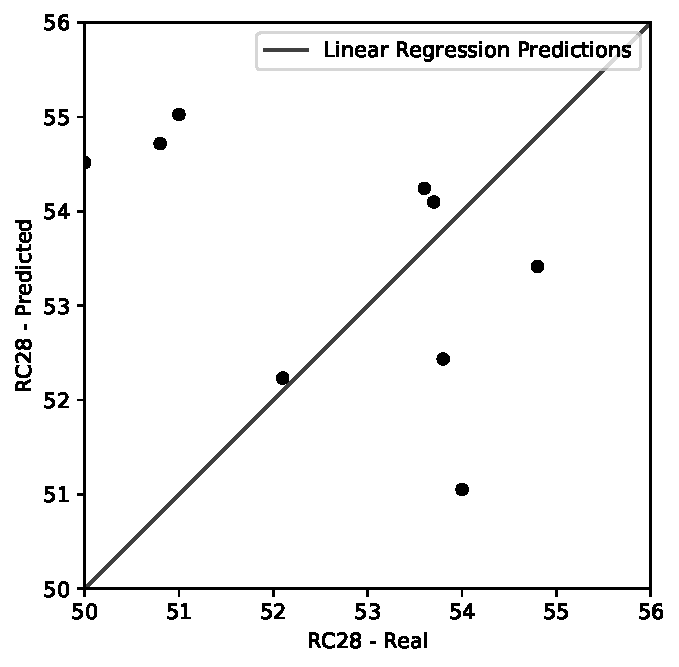
\includegraphics[width=.3\textwidth]{qq-LinearRegression.pdf} \hfill
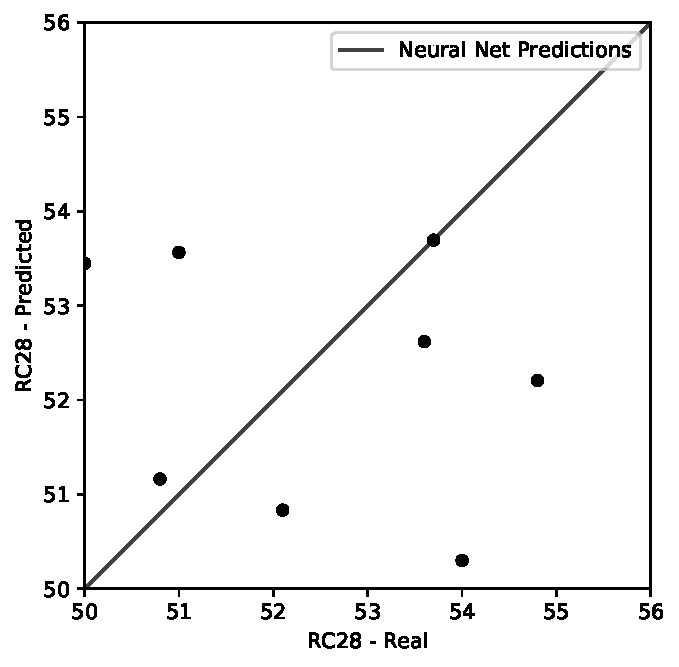
\includegraphics[width=.3\textwidth]{qq-NeuralNet.pdf} \hfill
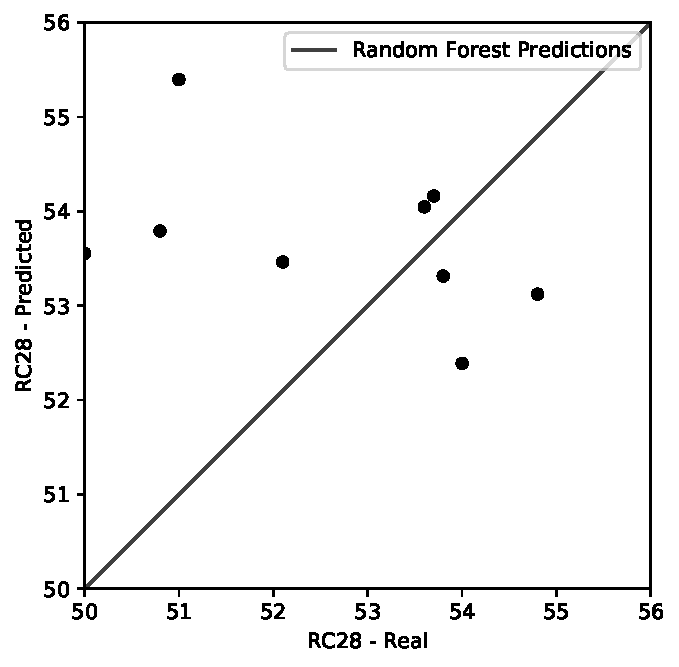
\includegraphics[width=.3\textwidth]{qq-RandomForest.pdf} 
\caption{Valores reais plotados contra os valores previstos para análise da distribuição aprendida por cada modelo} 
\label{fig:distr_lin}
\end{figure}

Para testar a acurácia de modelos em séries temporais, é comum se estudar o resíduo das
predições. 

\begin{figure}[H]
  \centering
  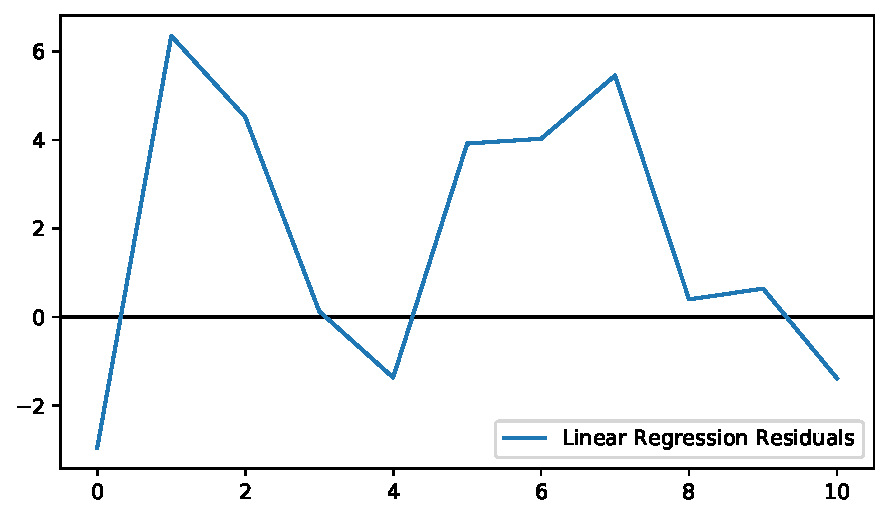
\includegraphics[width=.3\textwidth]{residuals-LinearRegression.pdf} \hfill
  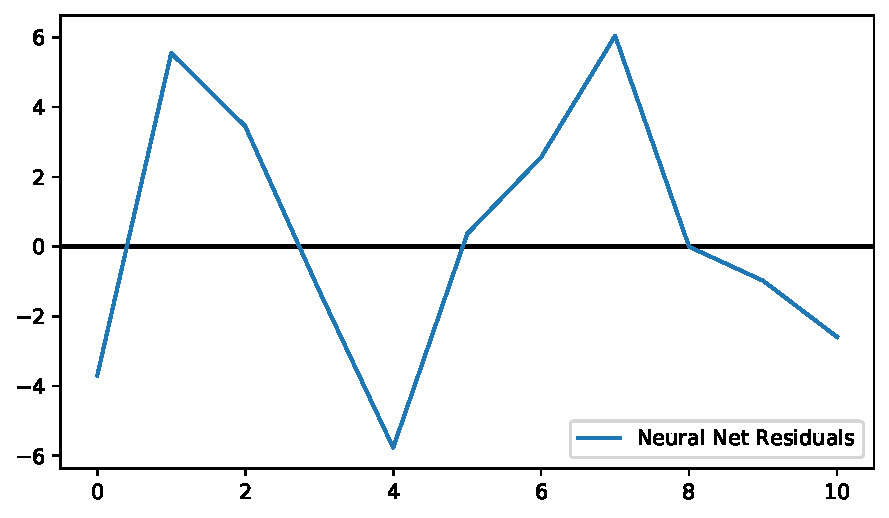
\includegraphics[width=.3\textwidth]{residuals-NeuralNet.pdf} \hfill
  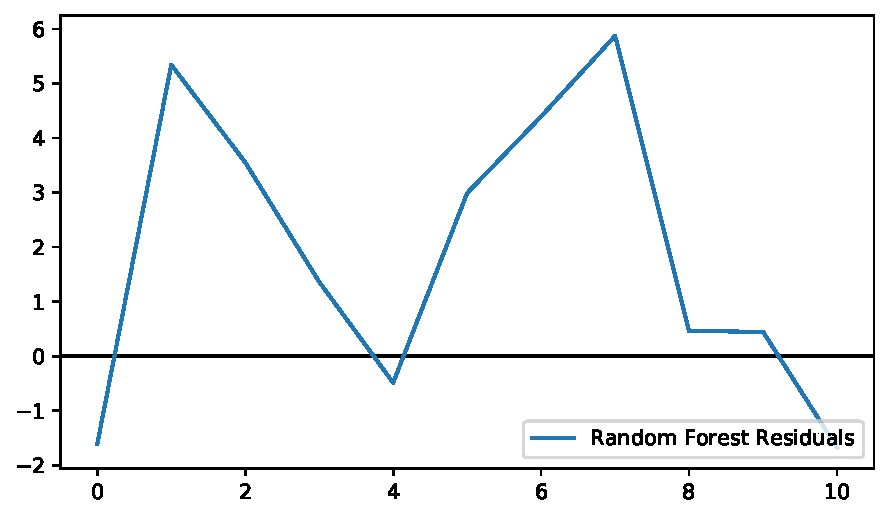
\includegraphics[width=.3\textwidth]{residuals-RandomForest.pdf} 
  \caption{Distribuição dos resíduos de cada modelo de Aprendizado Automático}
  \label{fig:res_lin}
\end{figure}

\subsection{Modelos de Séries Temporais}


Agora com um tratamento completo do problema como o de Aprendizado Automático para predição de séries
temporais, consideramos os dados sequencialmente, treinando e testando o modelo a partir de janelas de $w$
entradas consumidas em sequência pelo o modelo. A tarefa destes é então gerar
predições que continuem essa janela de dados. 

Como mencionado na introdução desse trabalho, um benefício das técnicas de
Aprendizado Profundo é a de escalar tarefas de aprendizado para datasets de
tamanho muito maior que era possível com modelos clássicos \citep{dlbook}.
Para tarefas de regressão de séries temporais, modelos recentes utilizam
diversas séries temporais de um mesmo processo simultaneamente.
Os modelos poderão então ter parâmetros tanto locais (calculados
para cada série) como globais (dividimos por todas as séries de treinamento).

\subsubsection{Divisão dos dados entre treino e validação}

Com o fim de explorar essa capacidade dos modelos de consumirem diversas séries
temporais, os dados da fábrica de Cajati foram separados por ano e consideramos
cada ano como um exemplo do processo a ser modelado, fornecendo-os separadamente
aos modelos. Os modelos de Aprendizado
Profundo irão então usar parâmetros locais para cada ano de produção de cimento,
mas globalmente buscar padrões para o funcionamento da fábrica. 

Para cada ano de 2012 até 2019 usaremos os primeiros 11 meses como dados de
treinamento e os últimos 30 dias como dados de validação.


\begin{figure}[H]
  \centering
  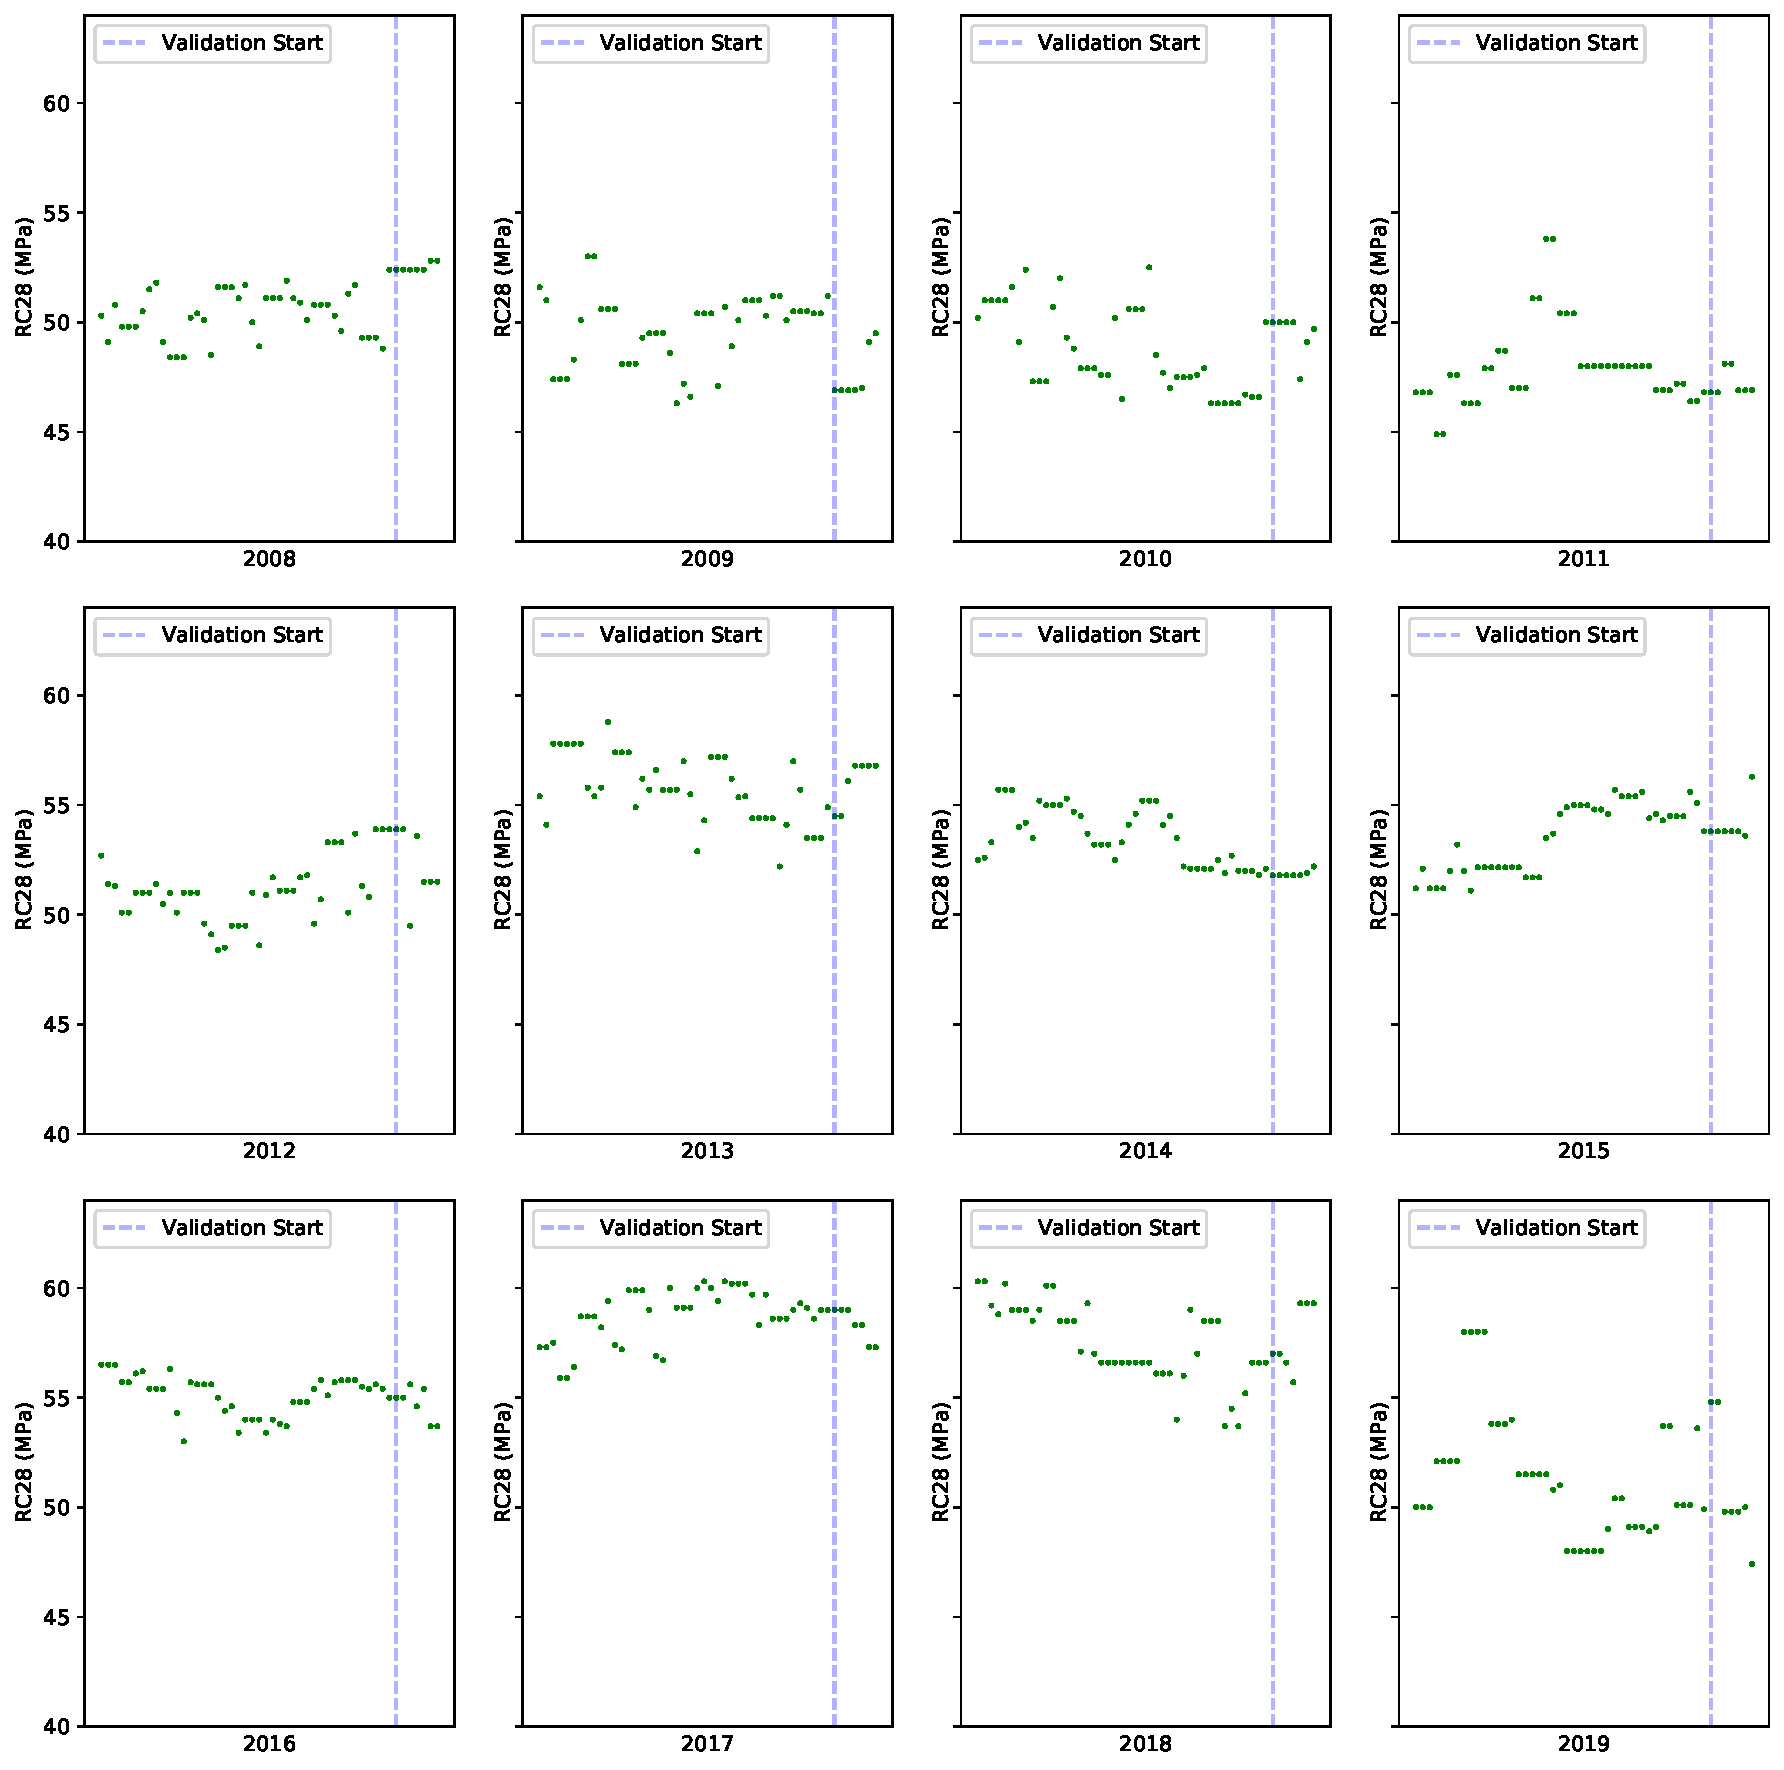
\includegraphics[height=.99\textwidth]{train_val_all_years.pdf} 
  \caption{Os dados são divididos em 11 datasets separados, onde temos por
    dataset 11 meses usados para treino e os últimos dias do ano para validação.} 
  \label{fig:trainvalallyears}
\end{figure}

\subsection{Regressão Linear Dinâmica com Filtragem Exponencial}

Com o fim de termos uma base de comparação para os modelos de
Aprendizado Profundo, aplicaremos o modelo proposto em \citep{grecialin}.
São criadas janelas de dados de treinamento e teste de maneira análoga a esse trabalho.

Usaremos 3 modelos com diferentes grupos de variáveis, a Tabela~\ref{tab:modelslin} mostra
as variáveis presentes em cada modelo, e o nome dado aos modelos pelo restante
desse trabalho. Também mostraremos resultados para o modelo corrigido
reglin\_ew, que é uma combinação dos modelos reglin\_1 e reglin\_7.


% copiar output do pandas aqui
% esta no notebook papergrecia
\begin{table}[]
\centering 
\begin{tabular}{llllllllllllll}
\toprule
reglin\_1 &  AGP &  AL2O3 &  SIO2 &  MGO &  IP &  FP &  SBL &  PF &  P2O5 &  FE2O3 &  RC1 &      &      \\
reglin\_3 &  AGP &  AL2O3 &  SIO2 &  MGO &  IP &  FP &  SBL &  PF &  P2O5 &  FE2O3 &  RC1 &  RC3 &      \\
reglin\_7 &  AGP &  AL2O3 &  SIO2 &  MGO &  IP &  FP &  SBL &  PF &  P2O5 &  FE2O3 &  RC1 &  RC3 &  RC7 \\
\bottomrule
\end{tabular}
\caption{O conjunto de variáveis usado para cada um dos modelos, de maneira análoga ao apresentado no trabalho \cite{grecialin}}
\label{tab:modelslin}
\end{table}

Os resultados para cada modelo no período de validação de cada ano são
reportados nas Figuras~\ref{fig:rc281preds},\ref{fig:rc283preds} e \ref{fig:rc287preds}.

\begin{figure}[H]
  \centering
  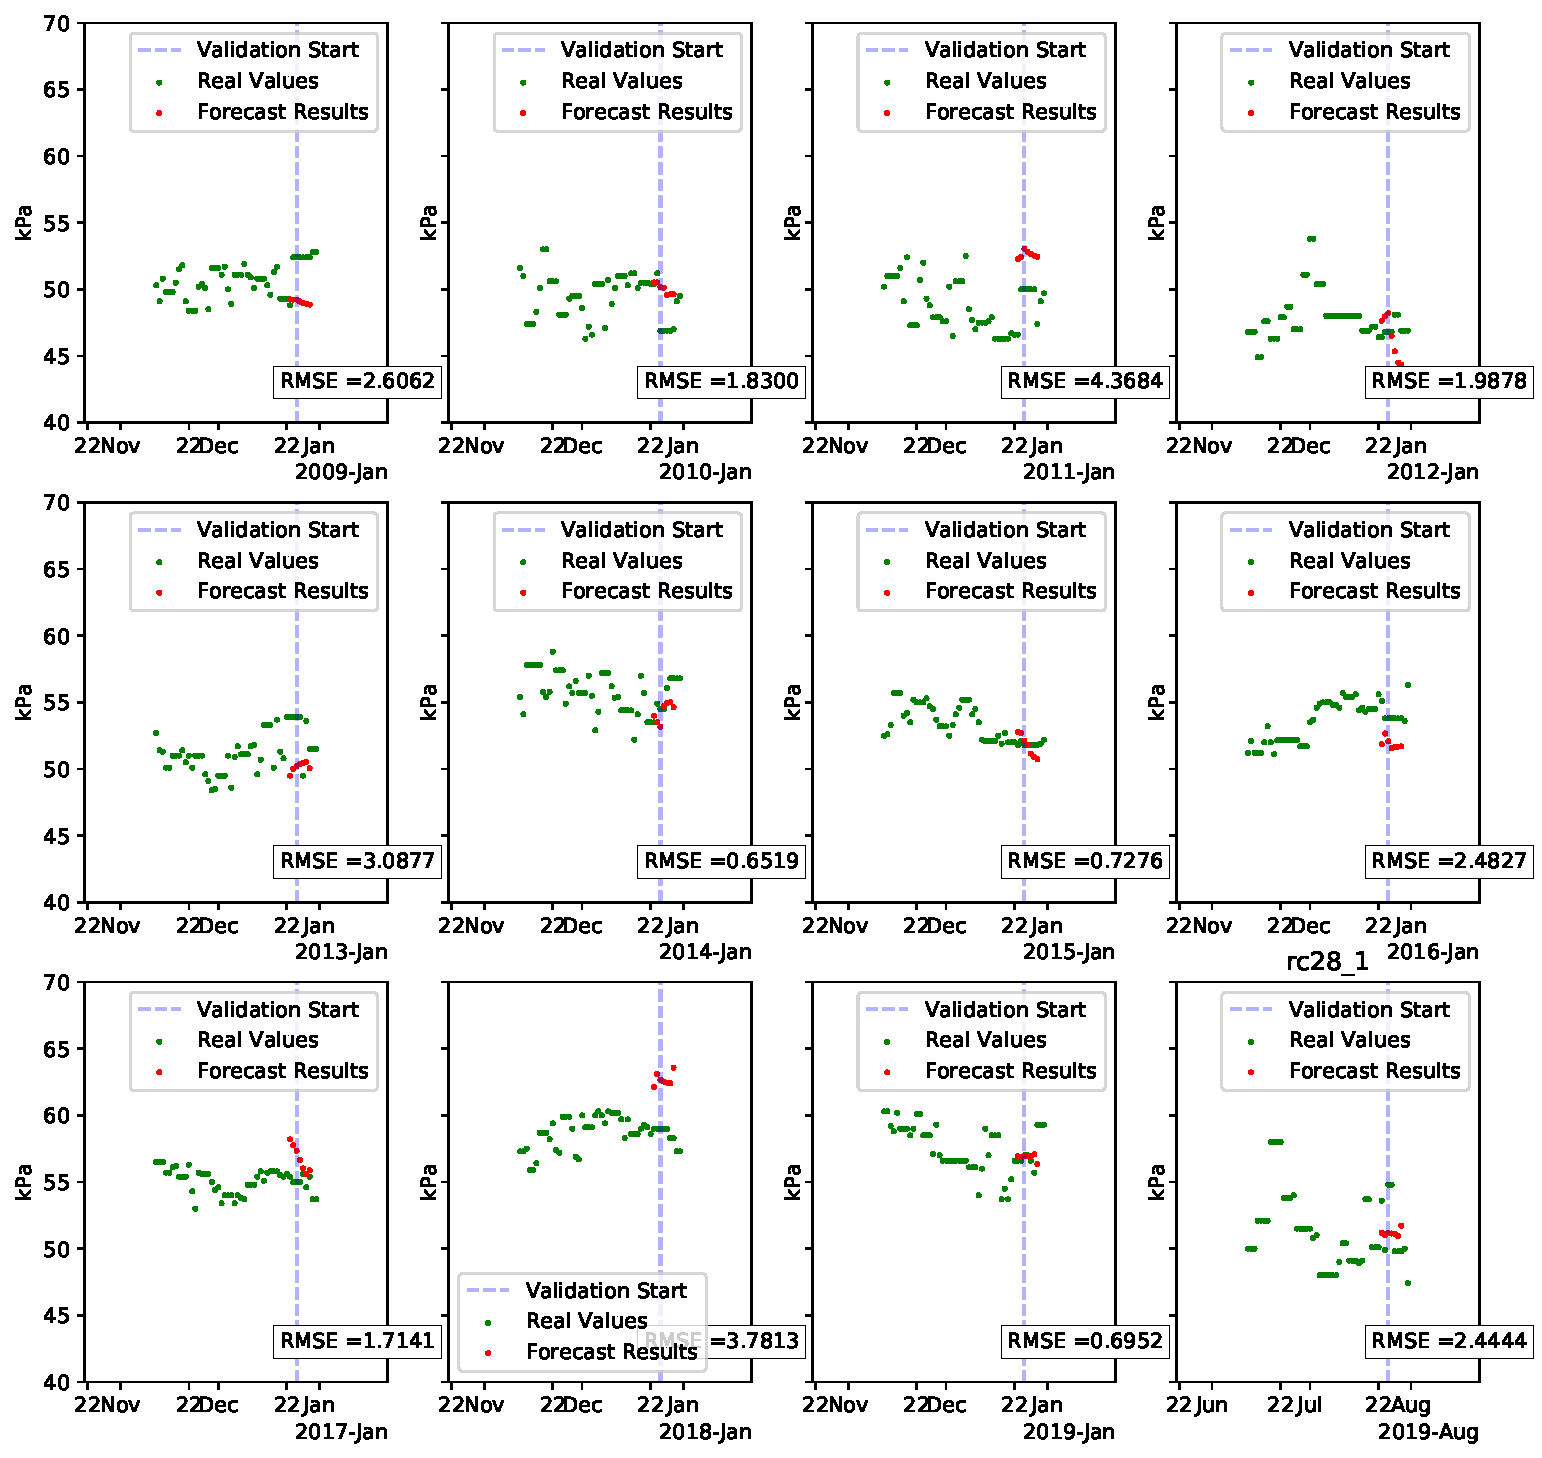
\includegraphics[width=0.6\columnwidth]{predgrecialin-rc28_1.pdf}
  \caption{Predições no período de teste para cada período de validação pelo
    modelo reglin\_1}
  \label{fig:rc281preds}
\end{figure}

\begin{figure}[H]
  \centering
  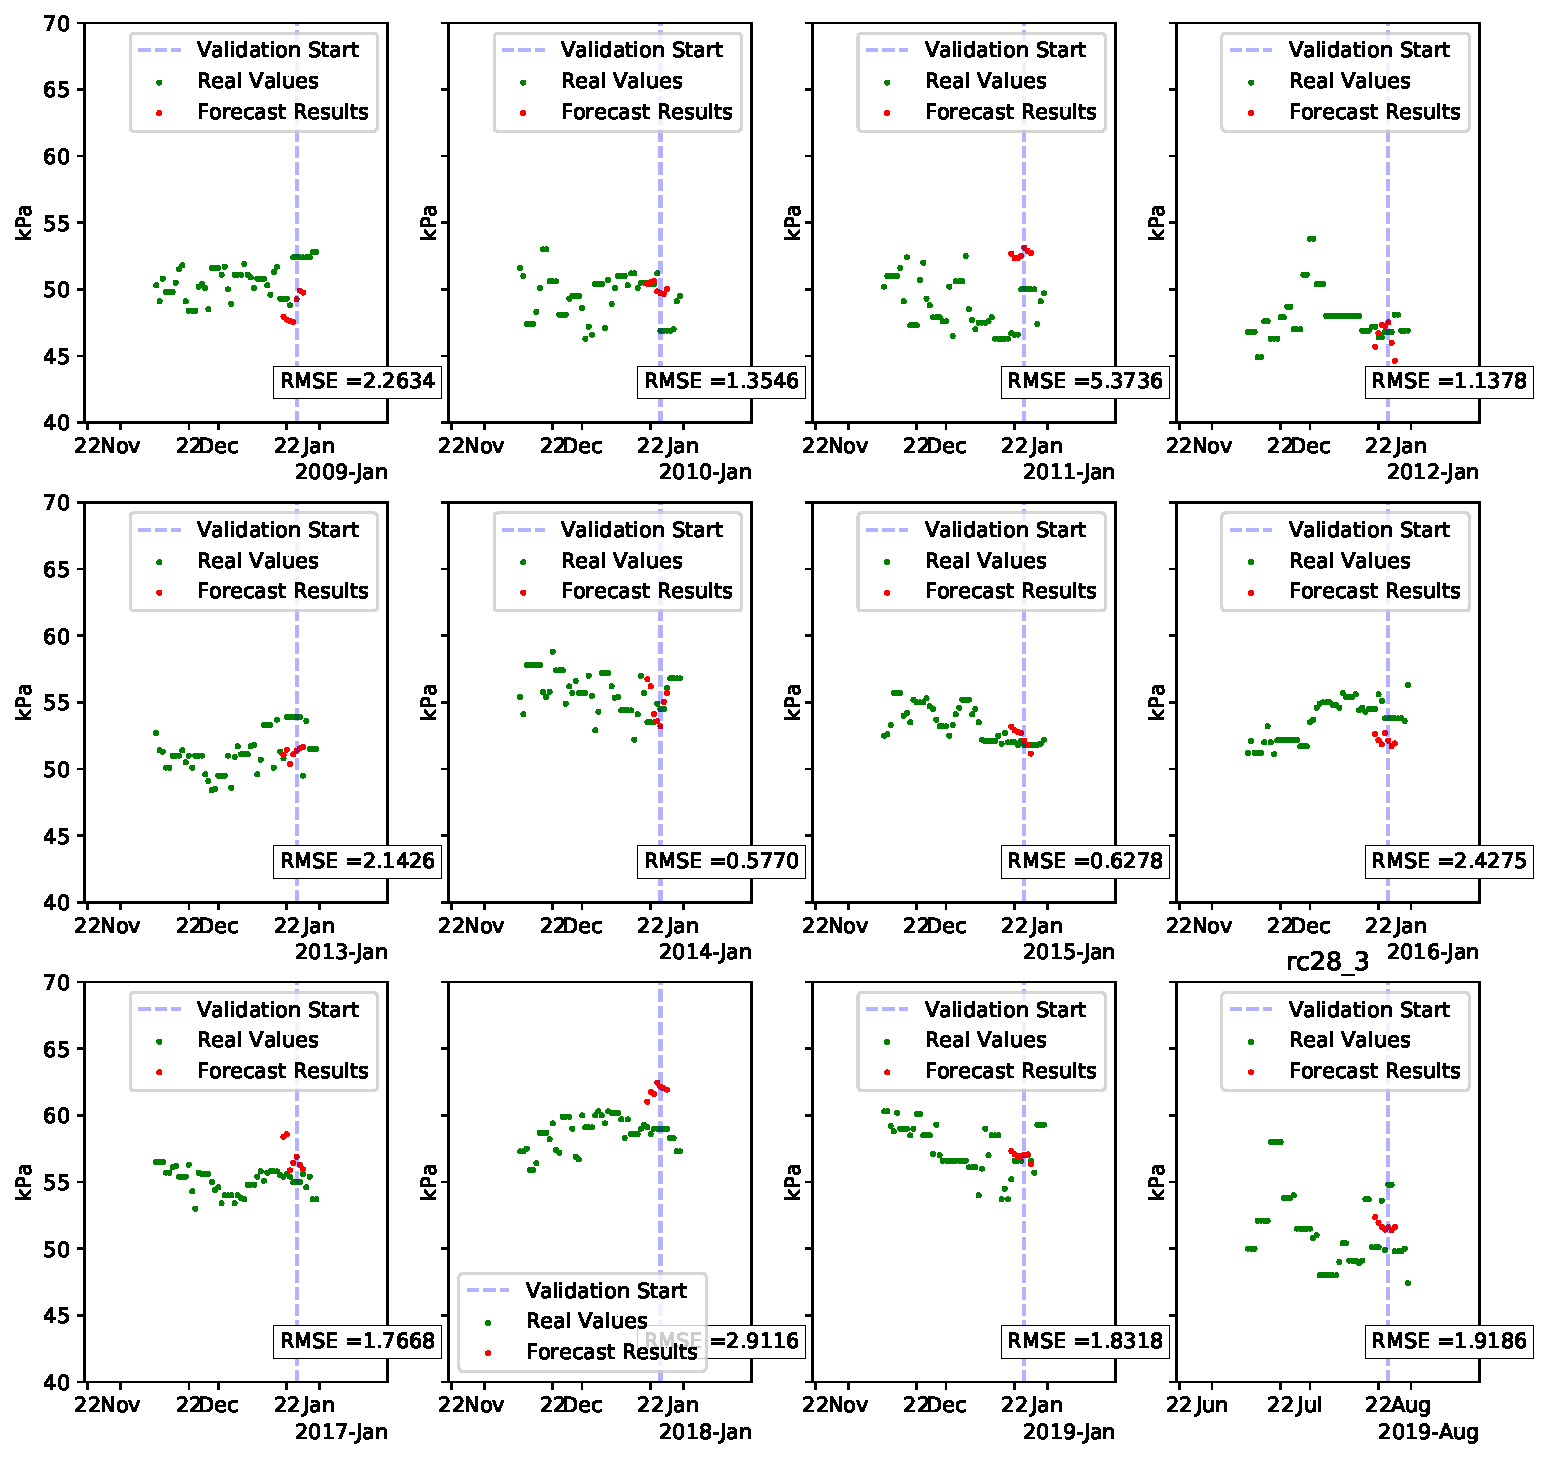
\includegraphics[width=0.6\columnwidth]{predgrecialin-rc28_3.pdf}
  \caption{Predições no período de teste para cada período de validação pelo
    modelo reglin\_3}
  \label{fig:rc283preds}

\end{figure}
\begin{figure}[H]
  \centering
  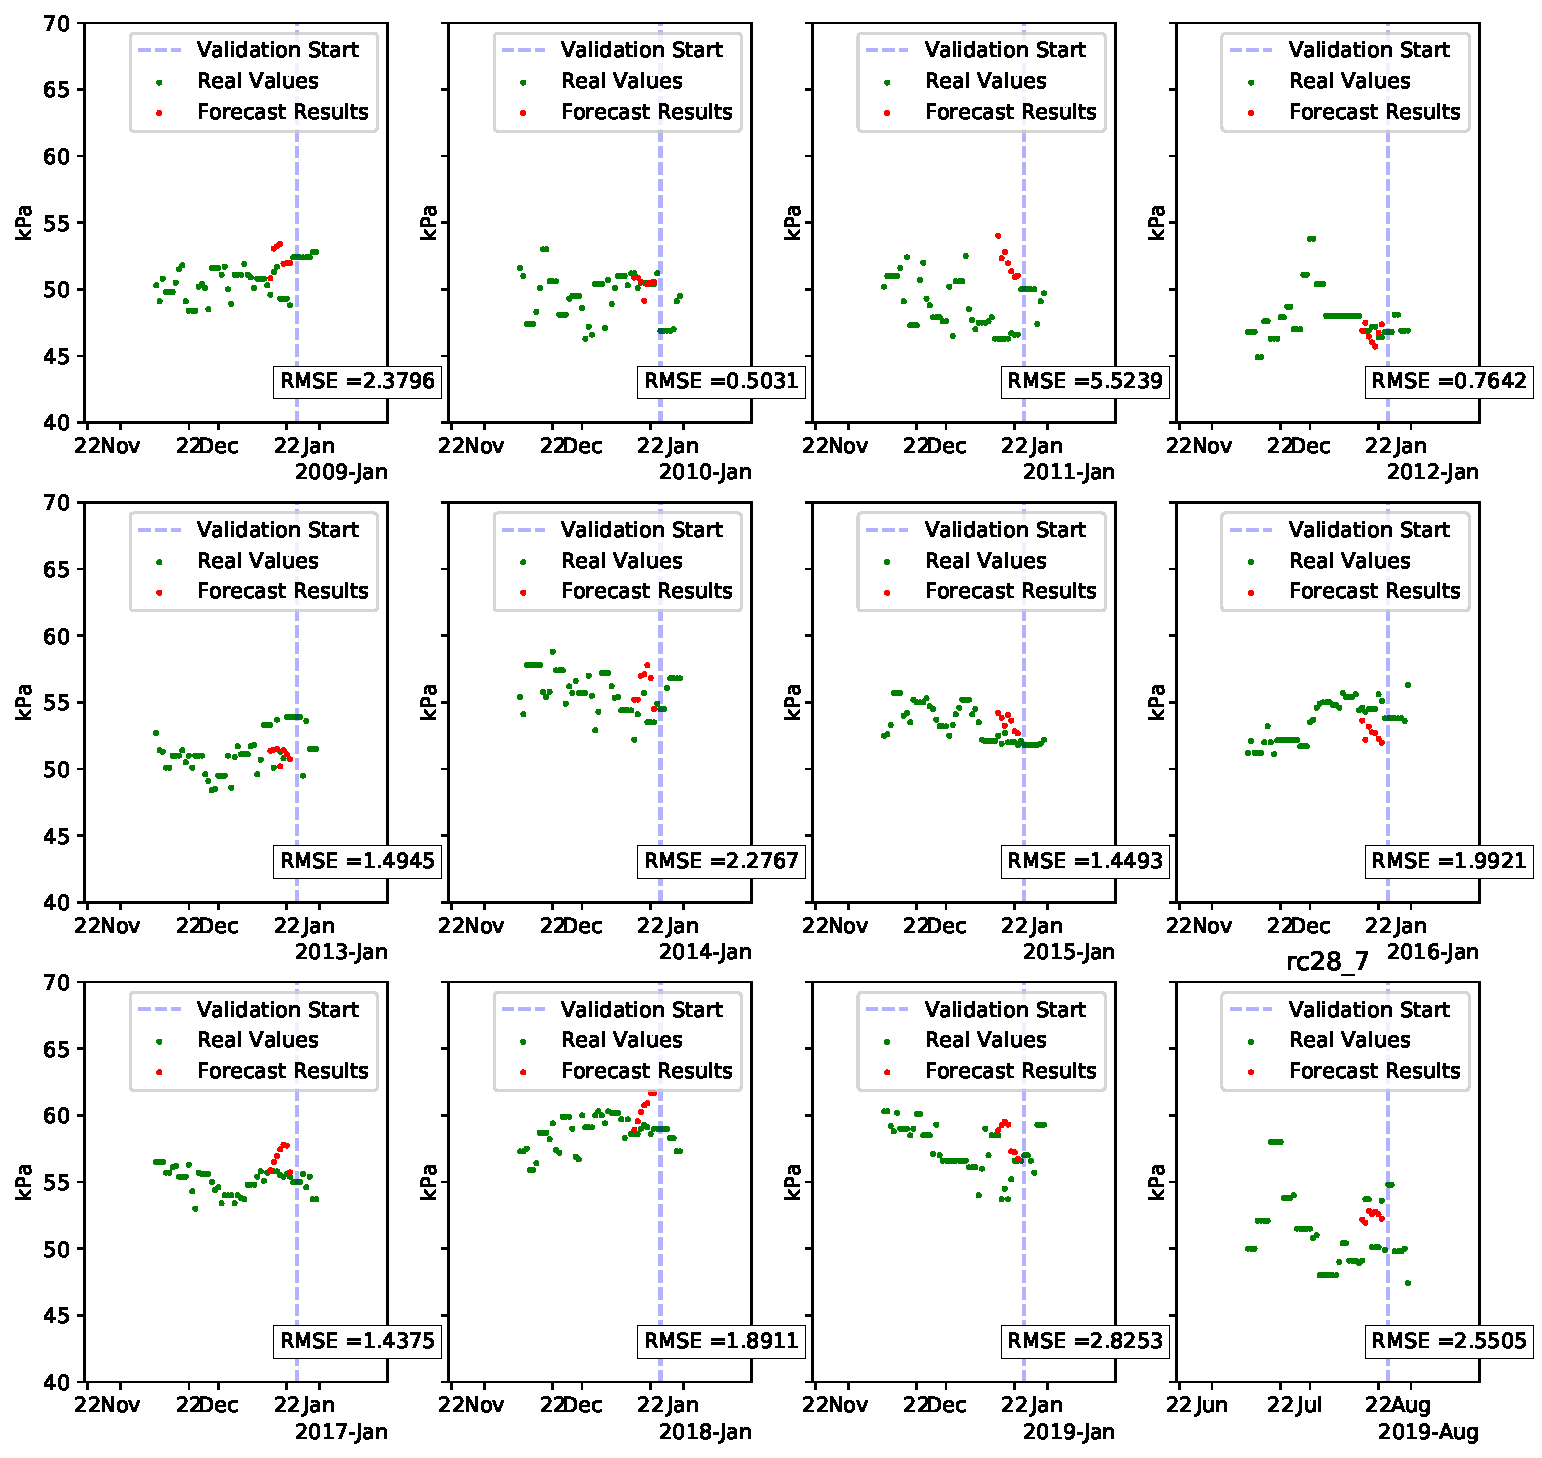
\includegraphics[width=0.6\columnwidth]{predgrecialin-rc28_7.pdf}
  \caption{Predições no período de teste para cada período de validação pelo
    modelo reglin\_7}
  \label{fig:rc287preds}

\end{figure}

Agregando esses valores, podemos apresentar o RMSE médio para cada modelo para
todo o dataset, para predições de 24h e 7 dias.

\begin{center}
  \begin{table}[]
    \centering
    \begin{tabular}{l|llll}
      \cline{2-3}
      & \multicolumn{1}{l|}{RMSE 24h} & \multicolumn{1}{l|}{RMSE 7 dias} &  \\ \cline{1-3}
      \multicolumn{1}{|l|}{reglin\_1} & 1.66                          & 2.19                             &  \\ \cline{1-1}
      \multicolumn{1}{|l|}{reglin\_3} & 2.12                          & 2.02                             &  \\ \cline{1-1}
      \multicolumn{1}{|l|}{reglin\_7} & 2.09                          & 1.63                             &  \\ \cline{1-1}
      \multicolumn{1}{|l|}{reglin\_ew} & 2.12                          & 1.42                            &  \\ \cline{1-1}
    \end{tabular}
    \caption{Valores agregados de RMSE para os modelos de Regressão Linear Dinâmica}

    \label{tb:rmse_exp}
  \end{table}
\end{center}



\subsection{Modelos de Deep Learning Bayesianos}


Usamos a implementação dos modelos DeepAR e DeepFactors da biblioteca GluonTS
\citep{gluonts}. O modelo Uber foi implementado com as primitivas fornecidas
pela biblioteca PyTorch \citep{pytorch}.

De modo análogo ao modelo de Regressão Linear Dinâmica, para
cada modelo de DL iremos treinar 3 versões distintas. Uma para cada conjunto de variáveis apresentado na Tabela~\ref{tab:modelslin}.


Para o modelo DeepAR, as versões treinadas serão chamadas de \textbf{DeepAR\_1},
\textbf{DeepAR\_3} e \textbf{DeepAR\_7}. Os outros modelos seguirão uma
regra de nomeação análoga.

As Figuras~\ref{fig:fordeepar1},\ref{fig:fordeepar3} e \ref{fig:fordeepar7} reportam as
predições geradas por cada versão do modelo DeepAR, bem como o intervalo de confiança. 

\begin{figure}[H]
  \centering
  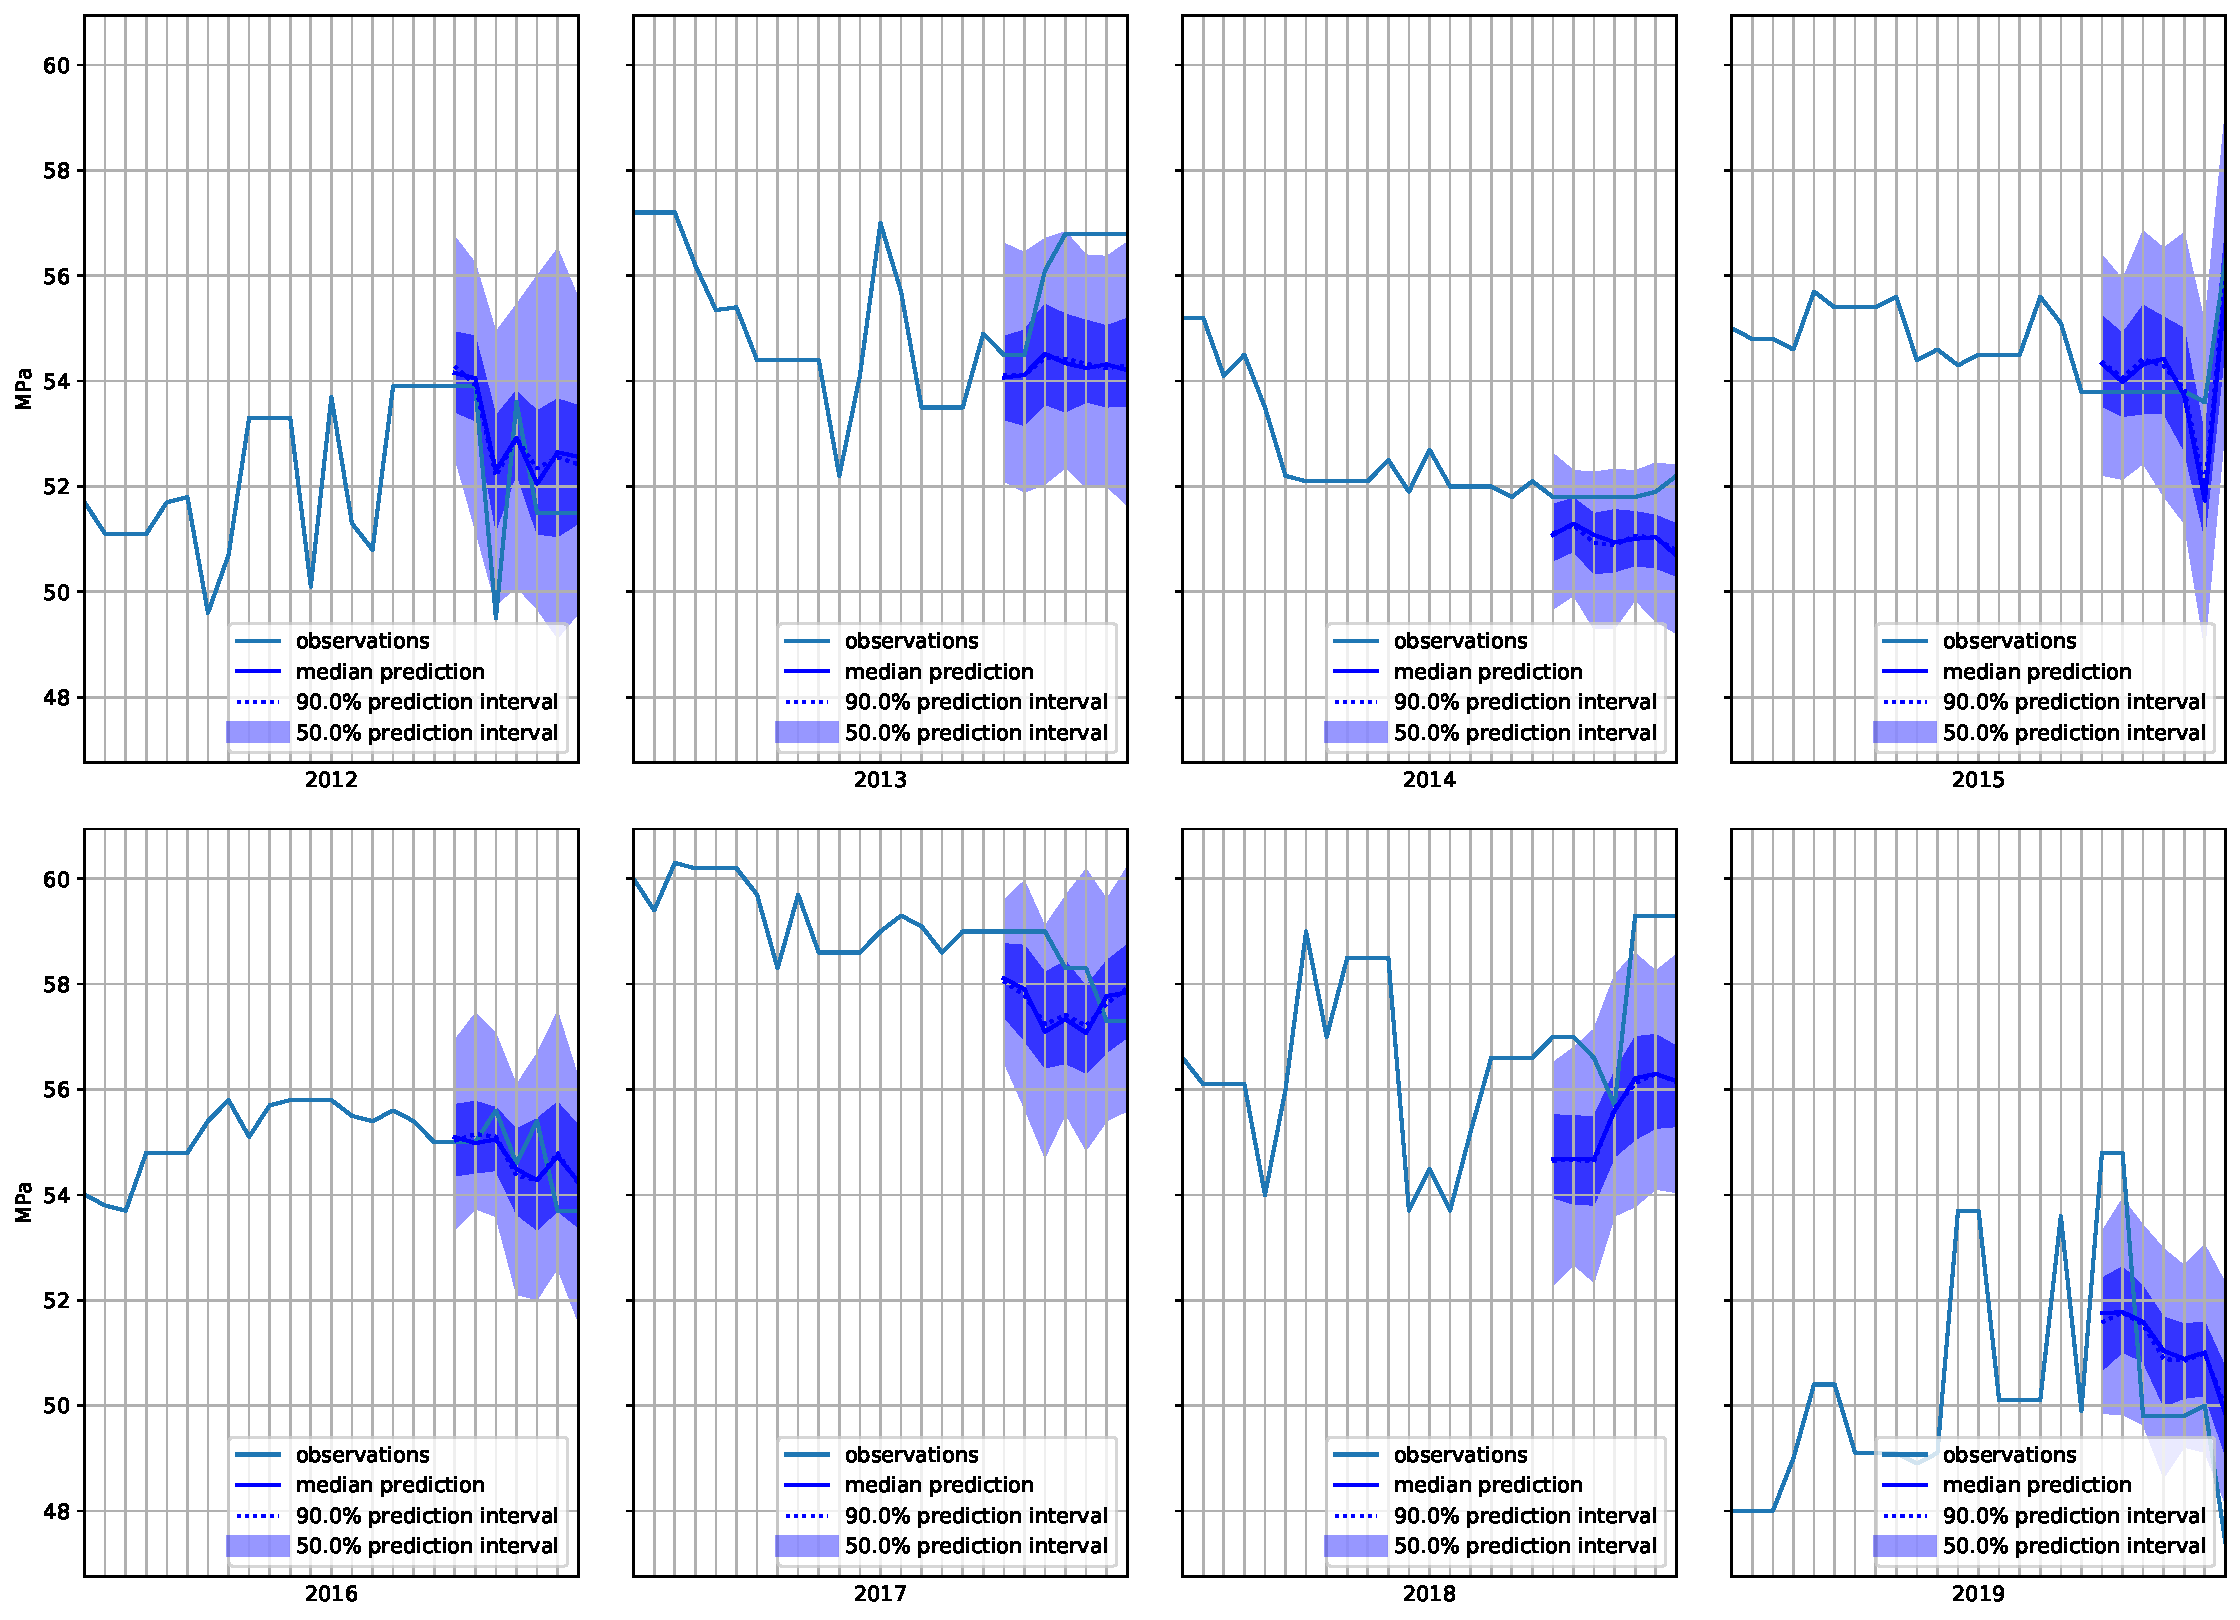
\includegraphics[width=.7\textwidth]{forecast_deep_ar1.pdf} 
  \caption{Predição para todos os dados de validação para o modelo DeepAR\_1}
  \label{fig:fordeepar1}
\end{figure}

\begin{figure}[H]
  \centering
  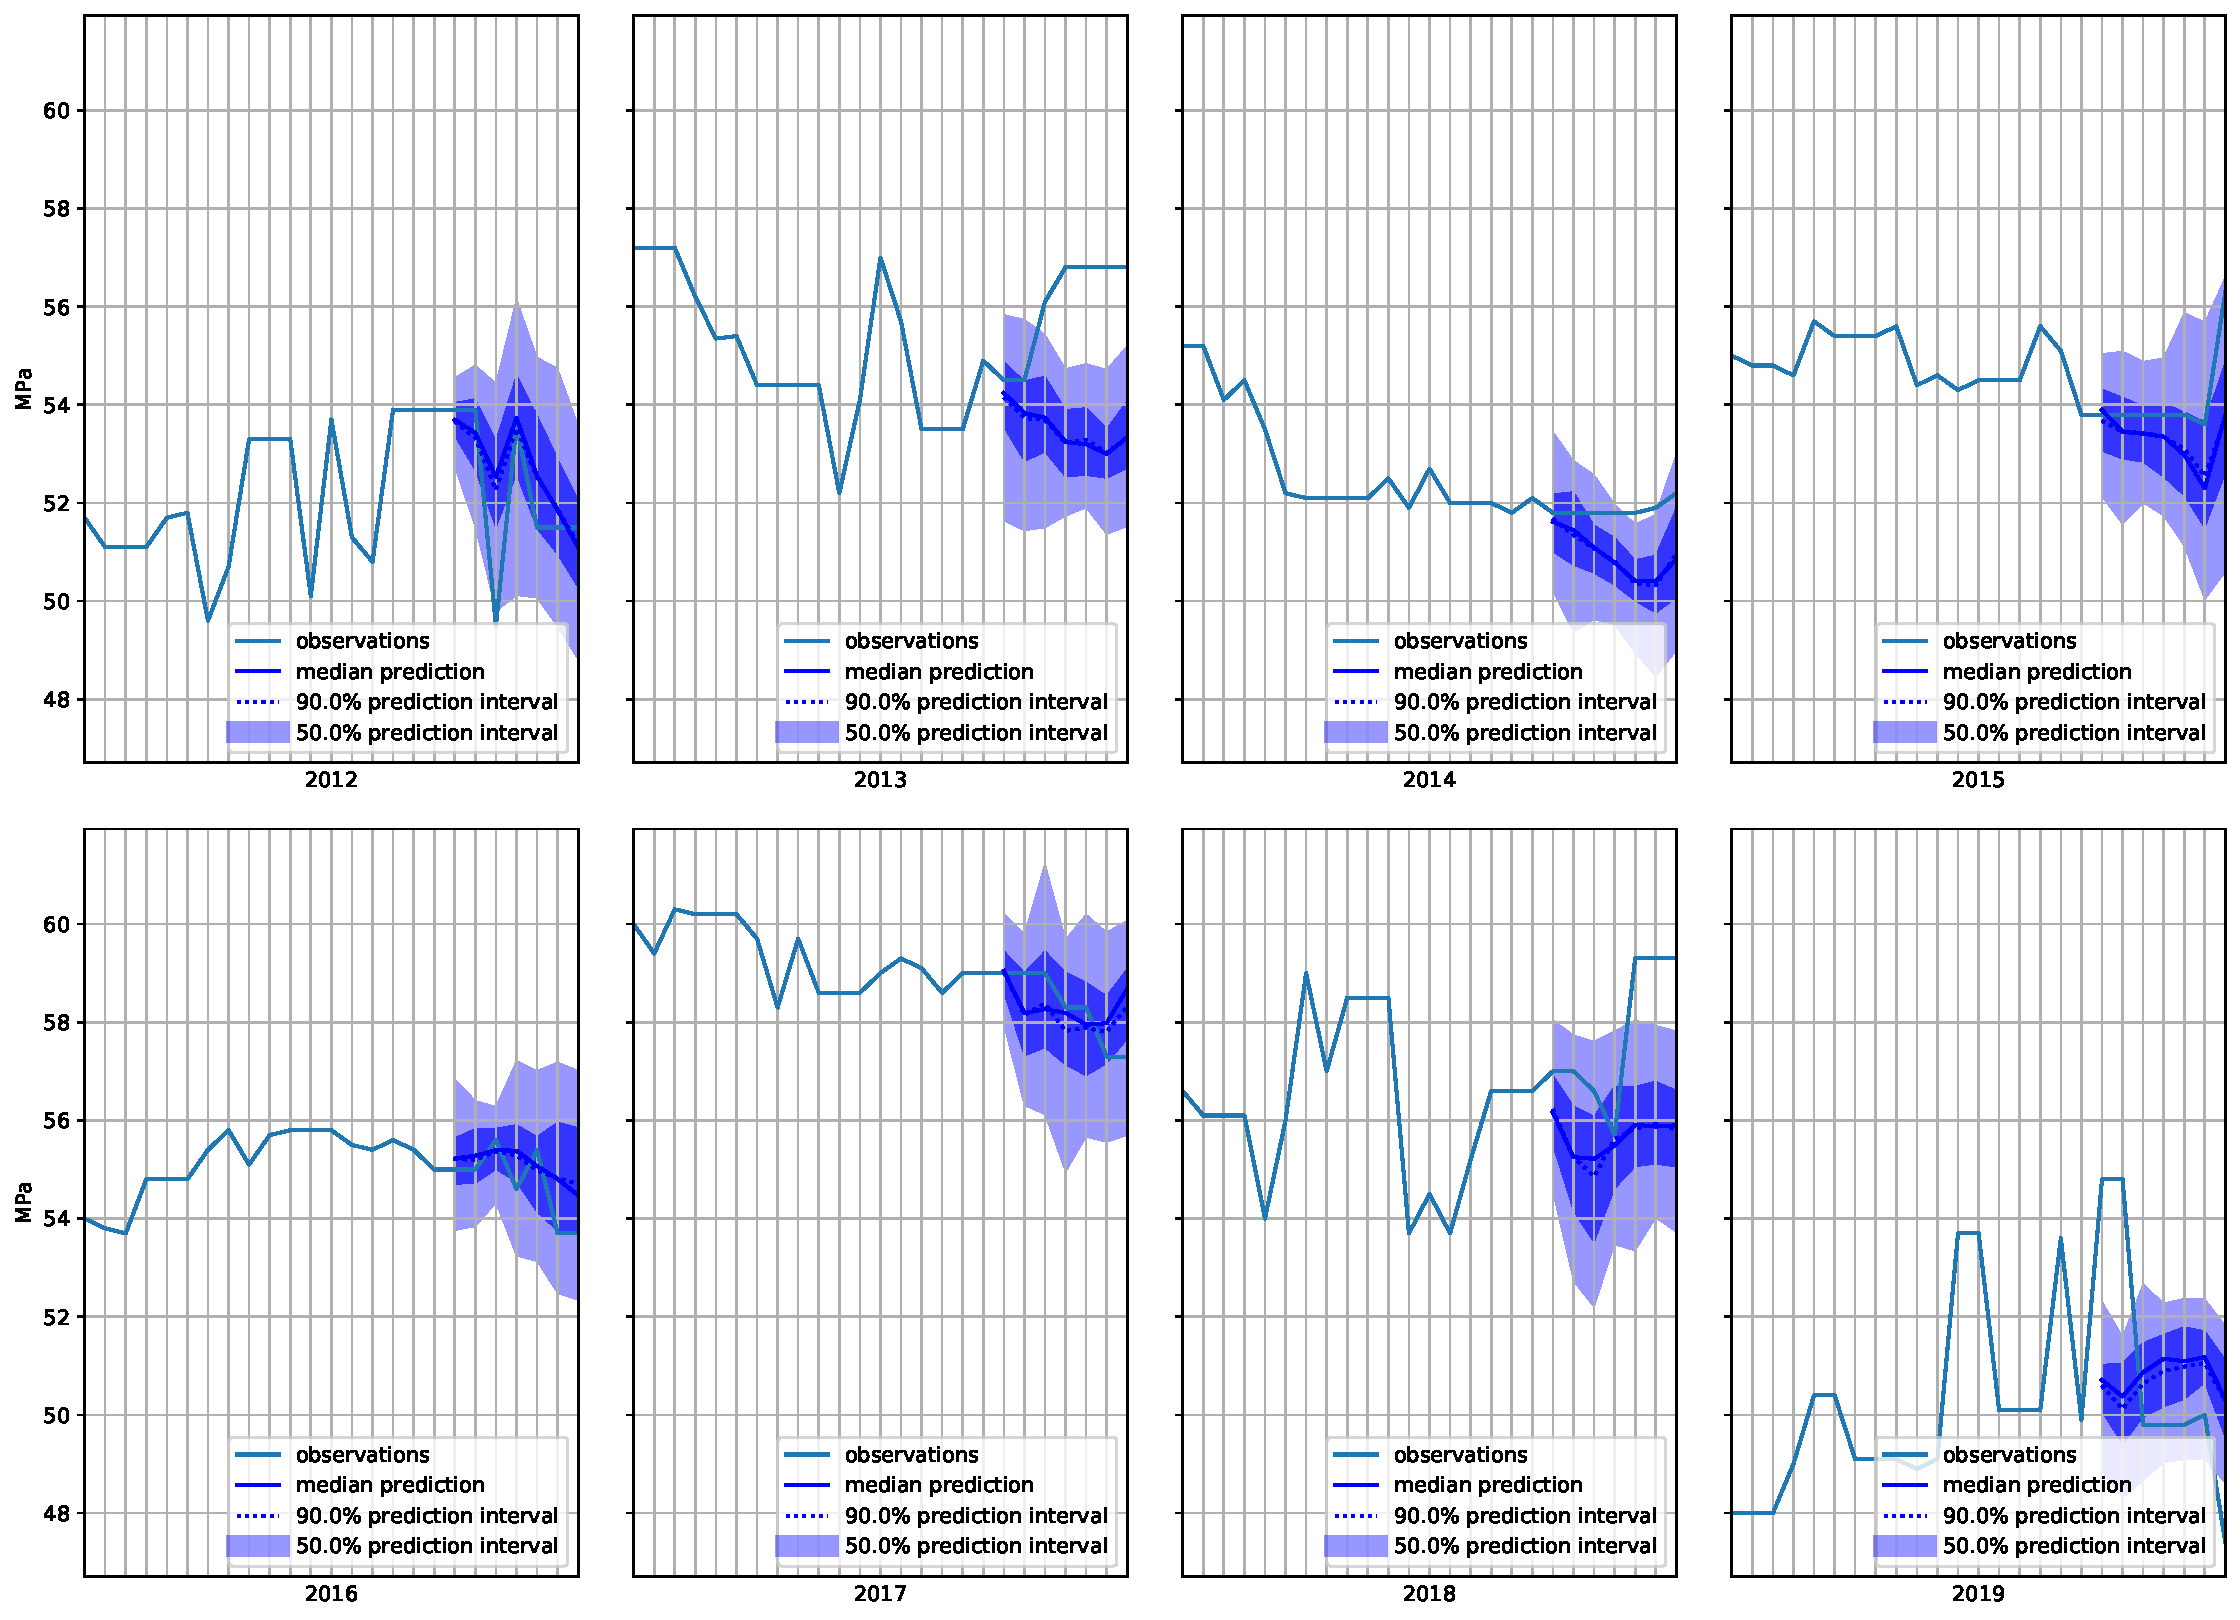
\includegraphics[width=.7\textwidth]{forecast_deep_ar3.pdf} 
  \caption{Predição para todos os dados de validação para o modelo DeepAR\_3}
  \label{fig:fordeepar3}
\end{figure}

\begin{figure}[H]
  \centering
  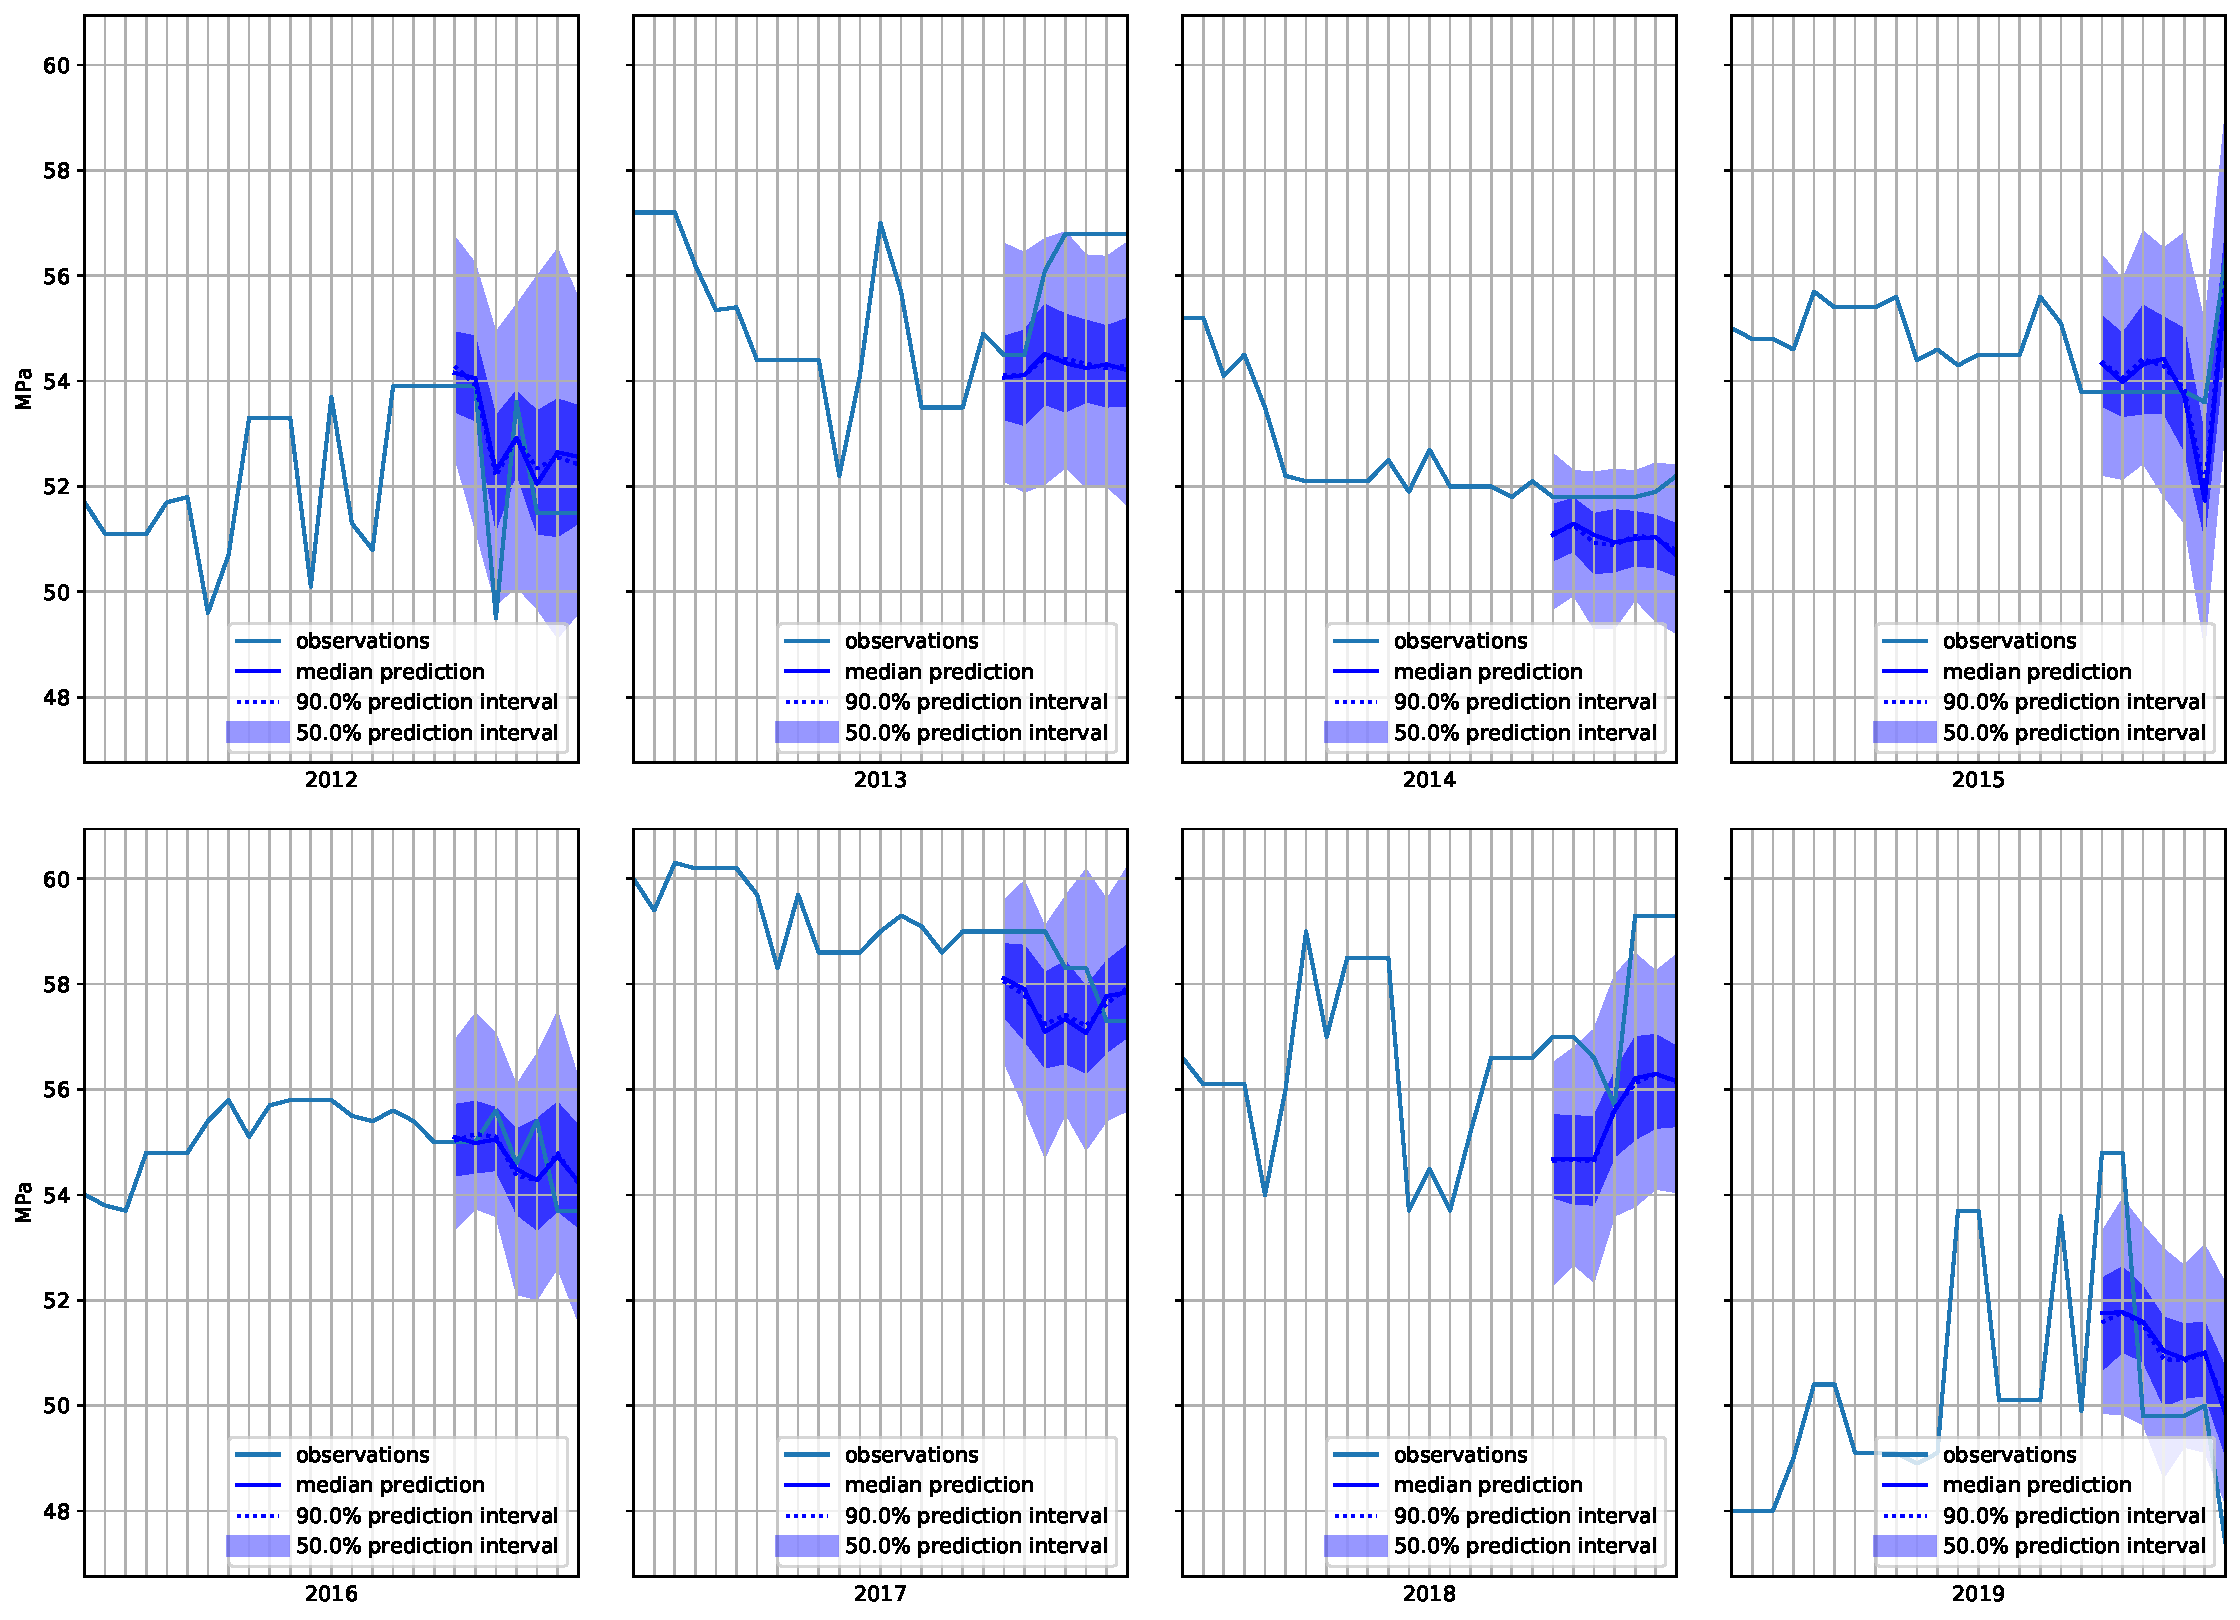
\includegraphics[width=.7\textwidth]{forecast_deep_ar7.pdf} 
  \caption{Predição para todos os dados de validação para o modelo DeepAR\_7}
  \label{fig:fordeepar7}
\end{figure}


Os modelos de Aprendizado Profundo Bayesianos retornam, para cada predição, uma distribuição de
probabilidade definida por média e variância, ou diversas realizações de uma
distribuição desconhecida, da qual podemos estimar esses parâmetros. 
Com o desvio-padrão podemos reportar o risco das predições para diversos percentis, como explicado na
Sessão~\ref{sec:quant}. Os custos quantílicos dos modelos são reportados na
Tabela~\ref{tb:quants}.


\begin{center}
\begin{table}
  \begin{tabular}{l|l|l|l|l|l|l|}
    \cline{2-7}
    & \multicolumn{3}{l|}{P50QL}                       & \multicolumn{3}{l|}{P90QL}                       \\ \cline{2-7} 
    & Factors\_7 & Factors\_3 & Factors\_1 & Factors\_7 & Factors\_3 & Factors\_1 \\ \hline
    \multicolumn{1}{|l|}{7d}  & 0.06           & 0.13           & 0.05           & 0.03           & 0.053          & 0.04           \\ \hline
    \multicolumn{1}{|l|}{24h} & 0.06           & 0.13           & 0.05           & 0.03           & 0.053          & 0.04           \\ \hline
    & Uber\_7 & Uber\_3 & Uber\_1 & Uber\_7 & Uber\_3 & Uber\_1 \\ \hline
    \multicolumn{1}{|l|}{7d}  & 0.02    & 0.23    & 0.02    & 0.018    & 0.015   & 0.013    \\ \hline
    \multicolumn{1}{|l|}{24h} & 0.01    & 0.21    & 0.01    & 0.012   & 0.010   & 0.008    \\ \hline
    & DeepAR\_7 & DeepAR\_3 & DeepAR\_1 & DeepAR\_7 & DeepAR\_3 & DeepAR\_1 \\ \hline
    \multicolumn{1}{|l|}{7d}  & 0.020     & 0.021     & 0.024     & 0.011     & 0.016     & 0.017     \\ \hline
    \multicolumn{1}{|l|}{24h} &  0.020     & 0.021     & 0.024     & 0.011     & 0.016     & 0.017     \\ \hline
  \end{tabular}
  \caption{Riscos-quantílicos para os percentis de 50\% e 90\% das distribuições
    das predições para os modelos de DL Bayesiano.}
  \label{tb:quants}
\end{table}
\end{center}


As versões do modelo DeepAR possuem em média os menores riscos. O que indica que
suas predições probabilísticas mais calibradas e com maior cobertura dos valores
reais observados.


A Tabela~\ref{tb:rmsetd} reporta o RMSE para cada modelo nos horizontes de tempo
estudados na modelagem.

\begin{center}
\begin{table}[]
  \begin{tabular}{l|l|l|l|}
    \cline{2-4}
    & DeepFactors\_7 & DeepFactors\_3 & DeepFactors\_1 \\ \hline
    \multicolumn{1}{|l|}{7d}  & 4.69           & 8.29           & 6.31           \\ \hline
    \multicolumn{1}{|l|}{24h} & 3.42           & 6.52           & 4.89           \\ \hline
    & Uber\_7        & Uber\_3        & Uber\_1        \\ \hline
    \multicolumn{1}{|l|}{7d}  & 2.70           & 2.51           & 2.21           \\ \hline
    \multicolumn{1}{|l|}{24h} & 1.62           & 1.73           & 1.44           \\ \hline
    & DeepAR\_7      & DeepAR\_3      & DeepAR\_1      \\ \hline
    \multicolumn{1}{|l|}{7d}  & 1.50           & 1.86           & 1.81           \\ \hline
    \multicolumn{1}{|l|}{24h} & 1.87           & 1.68           & 1.66           \\ \hline
  \end{tabular}
  \caption{Valores do RMSE para cada modelo nos horizonte de predição de 24h e 7 dias.}
  \label{tb:rmsetd}
\end{table}
\end{center}


\subsubsection{Versão corrigida do modelo DeepAR}

Também corrigimos o modelo \textbf{DeepAR\_1} com o modelo \textbf{DeepAR\_7} de maneira análoga a
Sessão~\ref{ses:ewma}, ao modelo corrigido damos o nome de \textbf{DeepAR\_ew}.

Usando a média retornada para cada predição dos modelos DeepAR, é possível
comparar o erro quadrático das predições de cada modelo. Iremos comparar esses resultados com os obtidos pelo modelo
linear dinâmico. Os modelos DeepAR consistentemente geram melhores predições agregando valores previstos por 7 dias
após a implementação do modelo em produção. As predições de 24h são naturalmente
ruidosas para todos os modelos testados nesse trabalho.

\begin{center}
\begin{table}[]
  \centering
  \begin{tabular}{l|llll}
    \cline{2-3}
    & \multicolumn{1}{l|}{RMSE 24h} & \multicolumn{1}{l|}{RMSE 7 dias} &  \\ \cline{1-3}
    \multicolumn{1}{|l|}{reglin\_1/DeepAR\_1} & 1.66 / 1.68                   & 2.19 / 1.75                      &  \\ \cline{1-1}
    \multicolumn{1}{|l|}{reglin\_3/DeepAR\_3} & 2.12 / 1.86                   & 2.02 / 1.68                      &  \\ \cline{1-1}
    \multicolumn{1}{|l|}{reglin\_7/DeepAR\_7} & 2.09 / 1.82                   & 1.63 / 1.42                      &  \\ \cline{1-1}
    \multicolumn{1}{|l|}{reglin\_ew/DeepAR\_ew} & 2.12 / 1.16                   & 1.42 / 1.12                      &  \\ \cline{1-1}
  \end{tabular}
  \caption{Valores do RMSE para cada modelo nos horizonte de predição de 24h e 7 dias.}
\label{tb:rmsedeepar}
\end{table}
\end{center}